\section{Neural Network Architecture}
\label{network_architecture}
Our neural network architecture for relation classification is based on \citet{nguyen2015}. We chose this architecture since it achieves the best results that we've encountered in contemporary research literature on SemEval 2010 Task 8, which would make our findings relevant to state-of-the-art research. This architecture is not appropriate for sequence labeling tasks however because of neural network components that are unique to the relation classification task as explained below. As a consequence, we use a related but slighter different architecture based on \citet{collobert2011} for the sequence labeling tasks and share neural network weights of the early layers between the two architectures.
\\\\
In the architecture described in \citet{nguyen2015} each word $s_i$ of an input sentence $s$ is first mapped to a word-vector $\vector{v}_i \in \mathbb{R}^d$ through a word-embedding matrix to form a sentence matrix $\vector{S}$. In our experiment, we initialize the word-embedding matrix with $d = 300$ dimensional GloVe vectors trained on the Common Crawl corpus (commoncrawl.org). To ensure that the dimensionality of $\vector{S}$ is consistent across sentences, we compute the longest sentence length $K$ of the sentences in the SemEval and ACE corpora and pad shorter sentences with a padding token as a preprocessing step, such that $\vector{S} = [\vector{v}_1, \dots, \vector{v}_K]^T$.

To indicate which words in the input sentence are the relation arguments, we compute the distance between each word index $i$ and the index of the first relation argument words $e1$ and $e2$ as $i - e1$ and $i - e2$ for the first and second argument respectively. These distances are mapped into real valued position vectors $\vector{p}_{1i}$ for the distance $i - e1$ for each word, and $\vector{P}_{2i}$ for the distance $i - e2$ for each word, both in  $\mathbb{R}^{d'}$. From these we construct the position matrices $\vector{P}_1 = [\vector{p}_{11},\dots,\vector{p}_{1K}]^T$ and $\vector{P}_2 = [\vector{p}_{21},\dots,\vector{p}_{2K}]^T$. We use the three matrices $\vector{S}$, $\vector{P}_1$ and $\vector{P}_2$ to form the augmented sentence matrix $\vector{S}' = [\vector{S} \mid \vector{P}_1 \mid \vector{P}_2] \in \mathbb{R}^{K \times (d + 2d')}$.
\\\\
The $K \times (d + 2d')$ dimensional augmented sentence matrix is used as input for a convolutional neural network layer. The convolution filters are applied over the full height of augmented sentence matrix in windows of $n$ tokens over the $K$ dimensional axis. In other words, each convolution filter is a weight matrix $\vector{W} \in \mathbb{R}^{n \times (d + 2d')}$. The output of the convolutional neural at position $i$ is:
$$
\sigma\left(w_0 + \sum\limits_{j = i}^{i + n}\vector{S}'_i\vector{W}_i^T\right)
$$
Where $\sigma$ is the rectified linear activation function, $\vector{W}_i$ and $\vector{S}'_i$ is the $i$'th row of the convolutional filter matrix and augmented sentence matrix respectively, and $w_0$ is a bias term. In our experiment we use 150 filters of each window size, and window sizes $n$ of 2, 3, 4 and 5 for a total of 600 convolutional filters.

We apply max-pooling to the output of each convolutional filter yielding a 600 dimensional feature vector, which is used as input for a soft-max output layer. See figure \ref{relation_architecture} for a diagram.
\\\\
For the sequence classification tasks we use a convolutional neural network architecture based on \citet{collobert2011}. This architecture is virtually identical to the architecture used for the relation classification task, with the exception of the position features. To predict the tag for word $s_i$ in the sentence $s$, a window of $K$ tokens around $s_i$ is transformed into a sentence matrix $\vector{S} = [\vector{v}_{i - \frac{K}{2}},\dots,\vector{v}_i,\dots,\vector{v}_{i + \frac{K}{2}}]^T \in \mathbb{R}^{K \times d}$ where $\vector{v}_i \in \mathbb{R}^d$ is taken from a word-embedding matrix. For words where $i \pm K / 2$ exceeds the sentence border a padding token is used. The sentence matrix $\vector{S}$ is used directly as input to the convolutional layer. In other words, the convolutional filter weights $\vector{W}$ for sequence classification tasks have dimensionality $n \times d$, where $n$ is the convolution filter window size.
\\\\
The subtle differences between the network architecture used for sequence and relation classification leads to some practical difficulties: Since most symbolic differentiation software used for neural network training such as TensorFlow or Theano use matrix-vector formulations of the convolution operation, neural network weights must be expressed as matrices in these frameworks \citep{abadi2016, theano2016}. This means that the convolutional filter weights $\vector{W}$ cannot easily be shared between the sequence classification tasks and the relation classification tasks, since the filters have dimensionality $n \times d$ in one and $n \times d + 2d'$ in the other.
\\\\
For this reason, we test three different strategies for for sharing neural network weights between the target and auxiliary tasks. Firstly, we test the enticingly simple strategy of \citet{collobert2008} and share only the word-embedding, and, when possible, the position-embedding matrix between the target and auxiliary tasks. 
\\\\
Secondly, extend the architecture of \citet{nguyen2015} to a \textbf{multi channel convolutional network} as introduced in \cite{kim2014}. The idea of a channel in this context is similar to a color channel in a digital image: An image is often represented as a stack of three matrices where each matrix component denotes color intensity in a color channel.
\\\\
We can use the idea of multi-channel convolutional neural networks to modify the architecture proposed by \citet{nguyen2015} to accommodate sharing convolutional filter weights between the networks for the target and auxiliary task. Specifically, we can produce two identical sentences matrices from an input sentence. One is used to produce the augmented sentence matrix, one is kept as is. We can feed the augmented sentence matrix into a task-specific convolutional layer, and the un-augmented sentence matrix into a convolutional layer that can be shared with auxiliary tasks.
\\\\
Thirdly, because the ACE 2005 relation classification task and SemEval 2010 Task 8 require exactly the same architecture, we can readily share both the embeddings and the convolutional filters over the augmented sentence matrix. We therefore test this weight sharing strategy as well, but only when using ACE 2005 as an auxiliary task. A diagram of neural network weights are shared between tasks can be seen in figure \ref{relation_sequence_weight_sharing}
\newpage
\begin{figure}[h!]
	\thispagestyle{empty}
	\begin{tikzpicture}[on grid]
    	\begin{scope}[yshift=0,
    				  every node/.append style={
	       	    	  	yslant=0.5,
    	    	        xslant=-1
		    	      },
    	              yslant=0.
    	              5,xslant=-1]
        	\fill[cyan,fill opacity=.9] (0,3.5) rectangle (5.5,5.5);
	        \draw[black,very thick] (0,0) rectangle (5.5,5.5);
	       	\fill[red,fill opacity=.7] (1,0) rectangle (2.5,5.5);
    	    \draw[step=5mm, black] (0,0) grid (5.5,5.5);
    \end{scope}
   	\begin{scope}[yshift=100,
   				  every node/.append style={
   	    	  	    yslant=0.5,
    	    	    xslant=-1
		    	  },
    	          yslant=0.
    	          5,xslant=-1]
        	\fill[white,fill opacity=.7] (0,0) rectangle (5.5,5.5);
        	\fill[red,fill opacity=.7] (1,4.5) rectangle (1.5,4);
	        \draw[black,very thick] (0,0) rectangle (5.5,5.5);
    	    \draw[step=5mm, black] (0,0) grid (5.5,5.5);
    \end{scope}
    \begin{scope}[yshift=160,
    			  xshift=0,
    			  every node/.append style={
	       	      	yslant=0.5,
    	    	    xslant=-1
		    	  },
    	          yslant=0.
    	          5,xslant=-1]
        	\fill[white,fill opacity=.9] (0,3) rectangle (5.5,2.5);
	        \draw[black,very thick] (0,3) rectangle (5.5,2.5);
    	    \draw[step=5mm, black] (0,3) grid (5.5,2.5);
    \end{scope}
    \begin{scope}[yshift=220,
    			  xshift=0,
    			  every node/.append style={
	       	      	yslant=0.5,
    	    	    xslant=-1
		    	  },
    	          yslant=0.
    	          5,xslant=-1]
        	\fill[white,fill opacity=.9] (0,3) rectangle (5.5,2.5);
	        \draw[black,very thick] (0,3) rectangle (5.5,2.5);
    	    \draw[step=5mm, black] (0,3) grid (5.5,2.5);
    \end{scope}
    \begin{scope}[yshift=-120, xshift=-100]
    	\draw[black,very thick] (0,0) rectangle (3,3.5);
   	    \draw[step=5mm, black] (0,0) grid (3,3.5);
    \end{scope}
        \begin{scope}[yshift=-100, xshift=15]
    	\draw[black,very thick] (0,0) rectangle (2,1);
		\fill[cyan,fill opacity=.9] (0,0) rectangle (2,1);
   	    \draw[step=5mm, black] (0,0) grid (2,1);
    \end{scope}
    \node [text width=4cm] at (7,1.8) {Augmented sentence matrix};
    \node [text width=3.5cm] at (7,-2.5) {Word and position embedding};
    \node [text width=4cm] at (7,-5.5) {Input sentence};
    \node [] at (3.5,.5) {Convolution filter};
	\node [text width=3.5cm] at (7,5) {Convolution output};
	\node [text width=4cm] at (7,9.5) {Max-pooling};
	\node [text width=4cm] at (7,12) {Soft-max};
	\node [] (input) at (0,-5.5) {\textit{A $[$woman$]_{e1}$ has been placed into the $[$house$]_{e2}$ as well.}};
	\node [] (output) at (0,13.5) {\textit{Entity-Destination(e1,e2)}};
	\node [text width=4cm] at (7,13.5) {Output};
	\node [] (start) at (0,11.5) {};
	\draw [-latex, thick] (input) edge (0, -4);
	\draw [-latex, thick] (start) edge (output);
	\end{tikzpicture}
	\caption{Diagram of the convolutional neural network for relation classification. The input sentence is mapped to a sentence matrix by concatenating the word-vector for each word in the word embedding matrix and the position-vector for each word-position in the position embedding matrix for both entities. The position embedding components of the architecture is shown in blue. This forms a $K \times d + 2d'$ matrix. Convolution filters are applied along the $K$-axis of the sentence matrix to produce the convolution output. Each element in the convolution output matrix corresponds to one convolution filter applied at one position of the sentence matrix. An example convolutional filter and its corresponding output unit is shown in red. Max-pooling is applied to the convolution output to obtain a feature-vector. This vector is used as input to a soft-max output layer.}
	\label{relation_architecture}
\end{figure}
\FloatBarrier
\newpage

\vspace*{1cm}

\tikzstyle{box} = [rectangle, draw, node distance=3cm, align=center, minimum height=4em, minimum width=18em, thick]
\begin{figure}[h!]
	\centering
	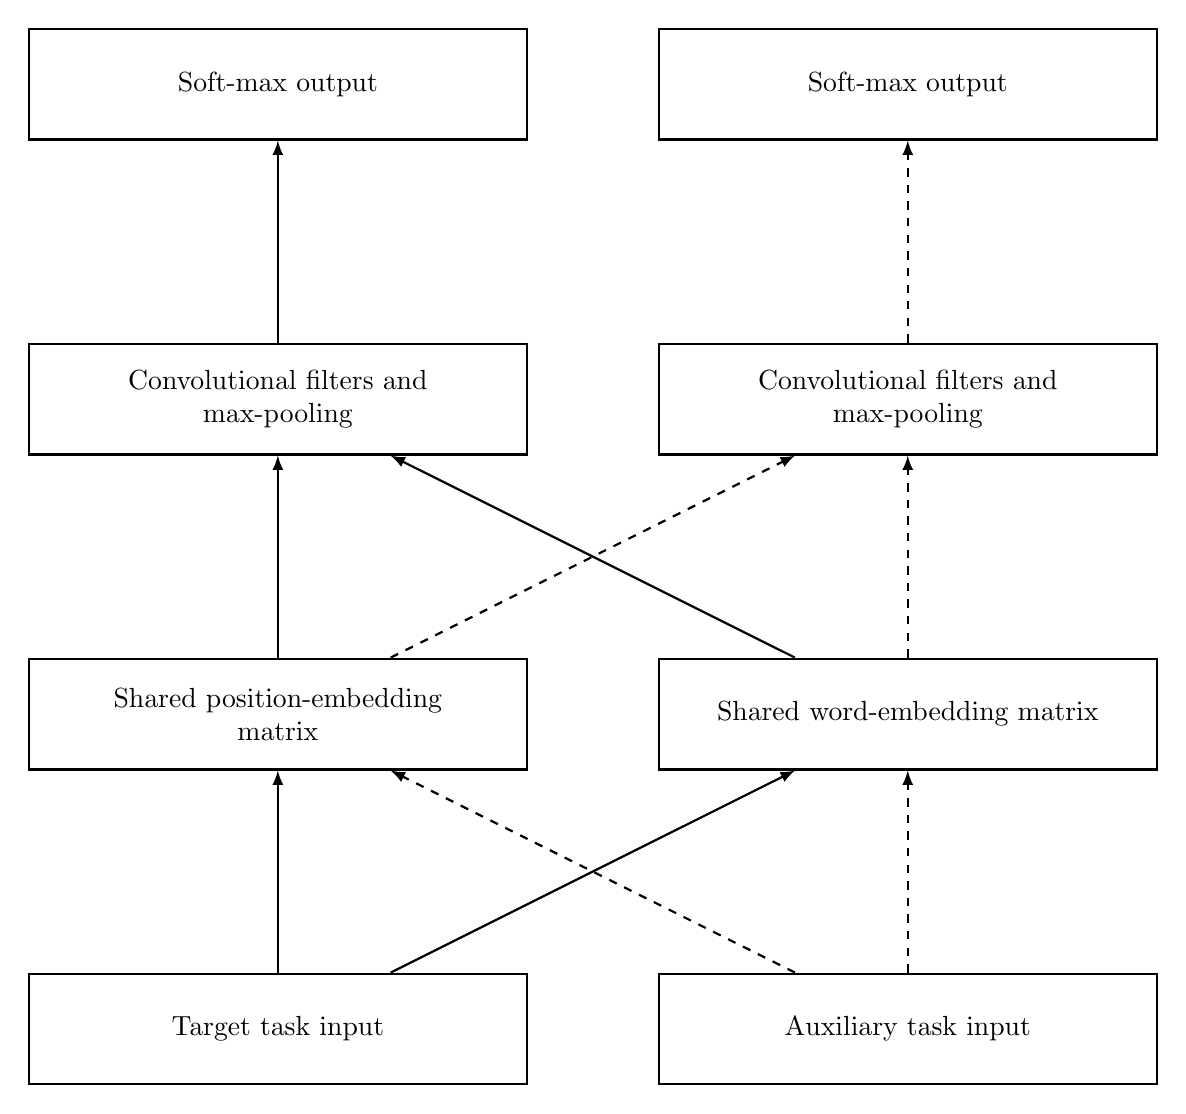
\begin{tikzpicture}
		\node [box] (embedding) at (4,0) {Shared word-embedding matrix};
		\node [box] (position_embedding) at (-4,0) {Shared position-embedding\\matrix};
		\node [box] (convolutions_task1) at (4,4) {Convolutional filters and\\max-pooling};
		\node [box] (convolutions_task2) at (-4,4) {Convolutional filters and\\max-pooling};
		\node [box] (output_1) at (4,8) {Soft-max output};
		\node [box] (output_2) at (-4,8) {Soft-max output};
		\node [box] (aux_sentence) at (4,-4) {Auxiliary task input};
		\node [box] (target_sentence) at (-4,-4) {Target task input};
		\draw[-latex, thick] (target_sentence) edge (embedding);
		\draw[-latex, thick] (target_sentence) edge (position_embedding);
		\draw[-latex, thick, dashed] (aux_sentence) edge (embedding);
		\draw[-latex, thick, dashed] (embedding) edge (convolutions_task1);
		\draw[-latex, thick] (embedding) edge (convolutions_task2);
		\draw[-latex, thick, dashed] (convolutions_task1) edge (output_1);
		\draw[-latex, thick] (convolutions_task2) edge (output_2);
		\draw[-latex, thick] (position_embedding) edge (convolutions_task2);
		\draw[-latex, thick, dashed] (aux_sentence) edge (position_embedding);
		\draw[-latex, thick, dashed] (position_embedding) edge (convolutions_task1);
		
	\end{tikzpicture}
	\caption{Diagram of the weight sharing strategy in which only the embedding matrices are shared between the auxiliary and target task. The solid lines show how network activations flow from the target task to the target output. Dashed lines show how the activations flow through the auxiliary network.}
	\label{relation_sequence_weight_sharing}
\end{figure}
\newpage
\tikzstyle{box} = [rectangle, draw, node distance=3cm, align=center, minimum height=4em, minimum width=18em, thick]
\begin{figure}[h!]
	\centering
	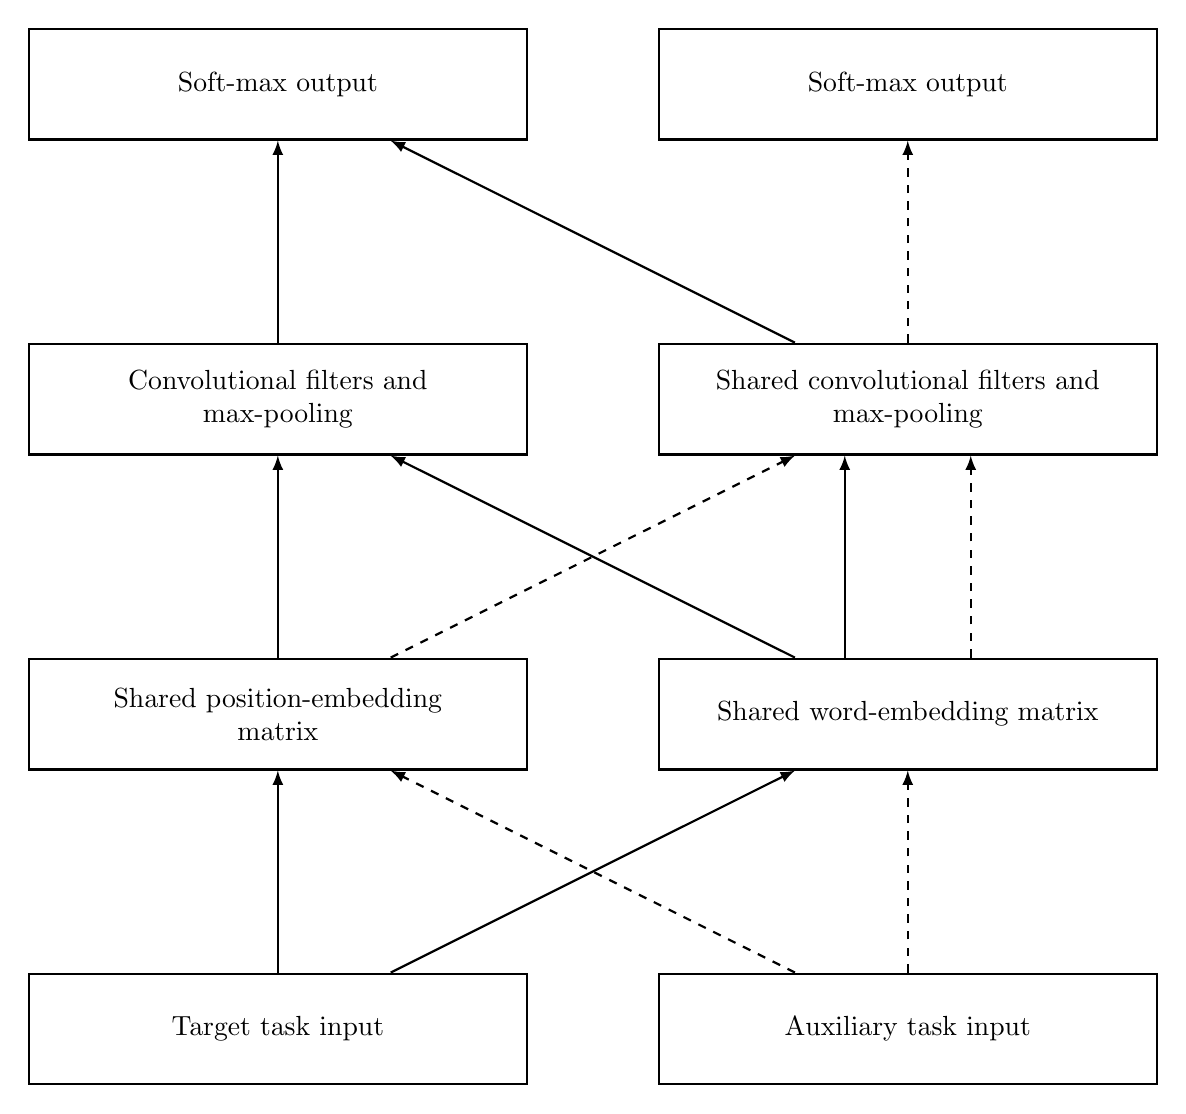
\begin{tikzpicture}
		\node [box] (embedding) at (4,0) {Shared word-embedding matrix};
		\node [box] (position_embedding) at (-4,0) {Shared position-embedding\\matrix};
		\node [box] (convolutions_task1) at (4,4) {Shared convolutional filters and\\max-pooling};
		\node [box] (convolutions_task2) at (-4,4) {Convolutional filters and\\max-pooling};
		\node [box] (output_1) at (4,8) {Soft-max output};
		\node [box] (output_2) at (-4,8) {Soft-max output};
		\node [box] (aux_sentence) at (4,-4) {Auxiliary task input};
		\node [box] (target_sentence) at (-4,-4) {Target task input};
		\draw[-latex, thick] (target_sentence) edge (embedding);
		\draw[-latex, thick] (convolutions_task1) edge (output_2);
		\draw[-latex, thick] (target_sentence) edge (position_embedding);
		\draw[-latex, thick, dashed] (aux_sentence) edge (embedding);
		\draw[-latex, thick, dashed, transform canvas={xshift=.8cm}] (embedding) edge (convolutions_task1);
		\draw[-latex, thick, transform canvas={xshift=-.8cm}] (embedding) edge (convolutions_task1);
		\draw[-latex, thick] (embedding) edge (convolutions_task2);
		\draw[-latex, thick, dashed] (convolutions_task1) edge (output_1);
		\draw[-latex, thick] (convolutions_task2) edge (output_2);
		\draw[-latex, thick] (position_embedding) edge (convolutions_task2);
		\draw[-latex, thick, dashed] (aux_sentence) edge (position_embedding);
		\draw[-latex, thick, dashed] (position_embedding) edge (convolutions_task1);
		
	\end{tikzpicture}
	\caption{Diagram of how neural network weights are shared when using a multi channel convolutional network to enable sharing convolutional filters. The solid lines show how network activations flow from the target task to the target output. Dashed lines show how the activations flow through the auxiliary network.}
\end{figure}
\FloatBarrier
